\documentclass[11pt]{ctexart}
\usepackage[margin=0.95in]{geometry}
\usepackage{amsmath,amssymb,amsthm}
\usepackage{booktabs}
\usepackage{tikz}
\usepackage{pgfplots}
\pgfplotsset{compat=1.18}
\usepackage{hyperref}
\hypersetup{hidelinks}

\newtheorem{definition}{定义}
\newtheorem{theorem}{定理}
\newtheorem{lemma}{引理}
\newtheorem{corollary}{推论}

\newcommand{\sig}{\operatorname{sig}}
\newcommand{\Indist}{\approx_{V}}
\newcommand{\Def}{\mathrm{Def}}
\newcommand{\Vocab}{\mathcal{V}}
\newcommand{\dom}{\mathcal{X}}
\newcommand{\Epos}{E^{+}}
\newcommand{\Eneg}{E^{-}}

\title{先词汇，后搜索：\\ 面向概念发现的查询驱动表征变更}
\author{}
\date{草稿---\today}

\begin{document}
\maketitle

\begin{abstract}
从少量例子中恢复一个未被明说的概念 $S$，是归纳的一项核心任务；然而概念分析、逻辑编程与
程序归纳，都只在给定的表征语言\emph{之内}搜索。尚无准则能判定：何时该更换的是表征，
而不是搜索。我们表明：当正例与反例在当前词汇下不可分辨时，没有任何可表达的假设与数据一致，
而追加例子只会增加约束；问题于是从“如何搜索”转为“该加入哪个谓词、需要多少代价”。我们为
这一步赋予类型：生成、闭包、表征变更、取证、控制这五类算子共享同一个状态与同一个度量，即
活假设的个数；四条定理确定了每一类能改变什么，因此表征变更与取证必须交替进行。提议成为一个
覆盖问题：贪心解与最优解相差在约 $15\%$ 以内。我们给出一个探索流程：模型提议谓词，程序询问
未决类的代表，oracle 负责裁决；该流程在每次回答错误率约 $20\%$ 以内保持可靠。两个负结果界定了
设计空间：对象级的查询选择是二阶的，而自适应噪声门会输给固定票差。总成本等于 $r/q$ 加上查询
轮数；核心结论已在 Lean~4 中机械化。当提议变得廉价时，成本趋于查询轮数，因此廉价的提议买到的
是更好的词汇，而不是更少的问题。
\end{abstract}

\section{引言}

从有限个例子做归纳，有两种熟悉的失败模式：搜索到不了目标，或者背景知识里没有这个模式。
第三种失败是逻辑的，不是计算的。目标概念可能无法在搜索所及的词汇上表达；此时假设空间里没有
任何一致元素，而在一种语言内部无论搜索多久，都产不出这门语言之外的句子。这种失败看起来像
证据不足，通常也被当作证据不足来报告，尽管再多的例子都去不掉它。

\textbf{贡献。} 我们给出关于“语言不足”的一个可判定判据（定理~\ref{thm:necessary}），并证明
追加例子无法修复它（定理~\ref{thm:monodata}）；一个推论指出，改写问题不能提供缺失的谓词
（推论~\ref{cor:rephrase}）。我们把谓词提议转化为覆盖问题，并测得贪心与最优相差在约 $15\%$ 以内
（定理~\ref{thm:cover}）。我们说明为什么仅凭一致性无法选出词汇（定理~\ref{thm:capacity}），
以及做出更好的选择需要多少查询代价（定理~\ref{thm:lower}）。我们在同一个度量上为五类算子
赋予类型（第~\ref{sec:operators}~节）：生成不能判定（定理~\ref{thm:gen}），闭包幂等
（定理~\ref{thm:clos}），取证是唯一严格减小者（定理~\ref{thm:ev}），词汇内部的重组打不破
撞车（定理~\ref{thm:recomb}），因此表征变更与取证必须交替（推论~\ref{cor:alt}）。我们给出
一个把提议、查询选择与裁决分开的探索流程，它在 oracle 错误率约 $20\%$ 以内保持可靠；并报告
两个界定设计空间的负结果：对象级的查询选择是二阶的，两个自适应噪声门都输给固定票差。
其中的数学大多属于形式概念分析与归纳逻辑编程的常识；本文的贡献在于把这份常识当作必要性判据
来用，以及由此得到的流程与基准。第~\ref{sec:operators}~节的定型是初等的，它的内容是消极的：
它排除“往固定词汇上不断加算子”或“反复重算一致性”并指望收敛的设计。

\textbf{我们不主张什么。} 我们没有提出新的学习算法，也不声称解决了“推断说话人到底想说什么”的
一般问题。谓词被假定具有可判定的成员关系；诸如“是一种自然类”这样的自然语言判断不在讨论范围内。
实证结果覆盖合成背景、一个小型代码域与一个 Lean 判定域；提议器接口的响应是手工填写的（流程里
没有真正的语言模型），因此除 $r/q$ 这套核算外，我们不对提议质量作任何断言。噪声保证在每次回答
错误率约 $0.2$ 以内成立；再高，我们所用的票差阈值就饱和了。

\section{相关工作}

\paragraph{形式概念分析。} 该框架固定属性集，从形式背景导出概念格 \cite{ganter1999}。属性探索
通过向专家询问蕴含关系来扩充属性集，是现有最接近我们形式化的程序；差别在于属性由专家提供、
每个成员问题由人回答，而我们让模型提议谓词（本文实验中由手工代填），oracle 只负责裁决。

\paragraph{归纳逻辑编程。} 归纳逻辑编程的实践者明确指出，约束瓶颈在语言偏置而非搜索：“即使对 ILP 专家，
确定合适的语言偏置也往往是令人沮丧且耗时的过程”，而自动识别合适的偏置“研究得很少”
\cite{cropper2021}。谓词发明能抬起词汇，但没有任何准则决定该发明哪个谓词。

\paragraph{理论形成与程序归纳。} Kemp 等人指出，“谓词发明至关重要，因为我们的目标之一就是
发现新概念，而指称这些概念需要新的谓词” \cite{kemp2010}。他们通过区分假设空间的计算意义
（一切可达状态）与心理意义（此刻在考虑的集合）来为固定假设空间辩护，并指出其搜索“常常会走到
与起点非常不同的区域”。这一辩护针对的是搜索轨迹；定理~\ref{thm:necessary} 表明，在固定词汇
内部的轨迹无法抵达词汇之外的概念。Kemp 与 Tenenbaum 在结构形式之间做选择 \cite{kemp2008}，但形式集合是预先给定的。DreamCoder 靠压缩生长出一个库 \cite{ellis2020}，那是被语料
而非被单次查询驱动的词汇变更。

\paragraph{结构映射、向量符号架构与细化。} 结构映射 \cite{falkenhainer1989} 与向量符号架构都固定了
关系词汇，只在其内部做映射或组合。反例引导的抽象精化（CEGAR）\cite{clarke2000} 在反例出现时
精化抽象，但反例由模型检查器产生并验证，而不是来自用户的成员查询。

\paragraph{模型空间的规格。} 主动推断把模型比较视为模型空间上的期望信息增益，并把该空间的
规格列为未决问题 \cite{friston2026}。贝叶斯的发展理论明确承认，学习者是在“已经存在的假设中
做选择” \cite{perfors2011}。两者都提供了本文借用的评分装置，但都没有提供触发条件。

\paragraph{自我纠错。} 一篇批判性综述没有找到仅靠提示反馈即可成功自我纠错的证据
\cite{kamoi2024}，这也是本流程把裁决者置于提议者之外的原因。

\paragraph{元推理与算子目录。} 元推理把“下一步算什么”当作一个关于该计算期望价值的决策问题
\cite{russell1991}。这条路线提供了第~\ref{sec:operators}~节里的控制类，但它假定了每个算子的
价值可估，且对该算子能改变什么保持沉默。定型正是缺失的前提：只有每一步对同一个度量的影响已知，
调度之间才可比较；而一旦证据与词汇固定，五类里有三类对势没有严格影响。

\paragraph{缺的是什么。} 在我们查阅的系统中，没有系统把“这些例子我们表达不了”当作可判定的触发条件，
决定\emph{该请求哪个}谓词，用廉价（且有噪）的 oracle 支付这笔开销，同时对会让新词汇
变得空洞的容量增长设上界。

\section{设定}\label{sec:setting}

\begin{definition}[词汇与签名]
设 $\dom$ 为有限对象集，$\Vocab \subseteq (\dom \to \{0,1\})$ 为有限谓词集。$x \in \dom$ 的
\emph{签名}定义为
\[
  \sig_{\Vocab}(x) \;=\; \lambda v.\; \begin{cases} v(x) & v \in \Vocab,\\ 0 & v \notin \Vocab.\end{cases}
\]
若 $\sig_{\Vocab}(x) = \sig_{\Vocab}(y)$，称两对象\emph{不可分辨}，记作 $x \Indist y$。
\end{definition}

\begin{definition}[可定义]
集合 $S \subseteq \dom$ 称为 \emph{$\Vocab$-可定义}，若存在布尔函数 $\varphi$，使得对所有 $x$
都有 $x \in S \iff \varphi(\sig_{\Vocab}(x)) = 1$。
\end{definition}

\begin{definition}[查询]
一次查询是一对互不相交的有限集 $Q = (\Epos, \Eneg)$。\emph{oracle}
$O \colon \dom \rightharpoonup \{0,1\}$ 回答成员问题；目标 $S$ 未知。oracle 不必是人：
它可以是测试套件、证明检查器、执行轨迹，或一个语言模型，而且一次调用可以回答一整批问题。
\emph{候选集}为
$\mathcal{F}_{\Vocab}(Q) = \{S : S \text{ 是 } \Vocab\text{-可定义的},\ \Epos \subseteq S,\ S \cap \Eneg = \emptyset\}$。
\end{definition}

\section{理论结果}

\begin{theorem}[刻画]\label{thm:char}
$S$ 是 $\Vocab$-可定义的，当且仅当 $S$ 是若干 $\Indist$-等价类之并，即
$\forall x\,y,\ x \Indist y \Rightarrow (x \in S \iff y \in S)$。
\end{theorem}

\begin{theorem}[必要性]\label{thm:necessary}
若存在 $x \in \Epos$、$y \in \Eneg$ 使 $x \Indist y$，则 $\mathcal{F}_{\Vocab}(Q) = \emptyset$。
\end{theorem}

\begin{corollary}[搜索无济于事]
在定理~\ref{thm:necessary} 的条件下，任何只在 $\Vocab$-可定义假设中搜索的算法，无论预算多大，
都无法返回与数据一致的概念。
\end{corollary}

\begin{figure}[t]
\centering
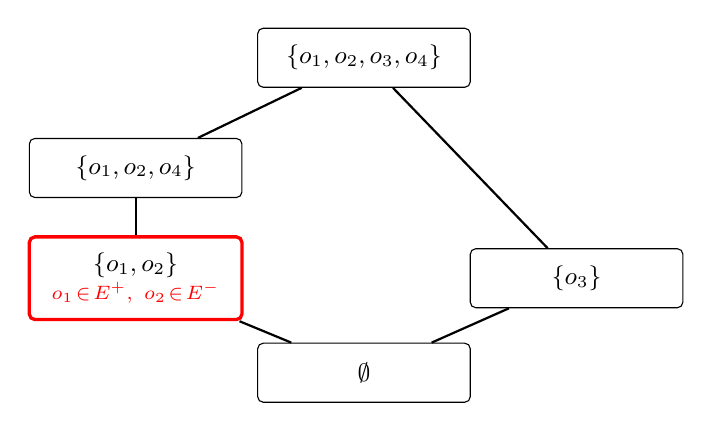
\begin{tikzpicture}[
  concept/.style={draw, rounded corners=2pt, minimum width=2.7cm, minimum height=0.75cm, font=\small, align=center},
  edge/.style={thick}
]
\node[concept] (top) at (0,4.0) {$\{o_1,o_2,o_3,o_4\}$};
\node[concept] (m1)  at (-2.9,2.6) {$\{o_1,o_2,o_4\}$};
\node[concept, draw=red, very thick, minimum height=1.05cm] (c) at (-2.9,1.2)
  {$\{o_1,o_2\}$\\[-1pt]{\scriptsize\color{red}$o_1\!\in\!\Epos,\ o_2\!\in\!\Eneg$}};
\node[concept] (m2)  at (2.7,1.2) {$\{o_3\}$};
\node[concept] (bot) at (0,0) {$\emptyset$};
\draw[edge] (top) -- (m1);
\draw[edge] (top) -- (m2);
\draw[edge] (m1) -- (c);
\draw[edge] (c) -- (bot);
\draw[edge] (bot) -- (m2);
\end{tikzpicture}
\caption{一个含两个属性的形式背景所对应的概念格。正例与反例落在同一个概念里，于是该节点之上或之下的每个
节点都同时包含二者或同时不包含：在这套词汇下不存在能分开它们的假设（定理~\ref{thm:necessary}），
在同一个格上加大预算也不会有任何改变。唯一的出路是加入一个能分开红框节点中那两个对象的属性。}
\label{fig:collision}
\end{figure}

\begin{theorem}[单调性]\label{thm:mono}
若 $\Vocab \subseteq \Vocab'$，则 $\approx_{\Vocab'} \;\subseteq\; \approx_{\Vocab}$。若谓词 $p$
能分开 $x$ 与 $y$，则 $x \not\approx_{\Vocab \cup \{p\}} y$。
\end{theorem}

\begin{theorem}[容量]\label{thm:capacity}
令 $m = |\{\sig_{\Vocab}(x) : x \in E\}|$。$\Vocab$-可定义集在 $E$ 上的不同限制至多
$2^{m}$ 个。
\end{theorem}

\begin{theorem}[更多数据不修复词汇]\label{thm:monodata}
若 $\mathcal{F}_{\Vocab}(Q) = \emptyset$，则对任何正例集包含 $\Epos$、反例集包含 $\Eneg$ 的
查询 $Q'$，都有 $\mathcal{F}_{\Vocab}(Q') = \emptyset$。并且随着例子增加，候选集只会缩小：
追加的例子能暴露词汇不足，但永远不能修复它。
\end{theorem}

\begin{corollary}[改写问题不能分离]\label{cor:rephrase}
在模型中，一个问题就是对某个对象做成员测试，措辞不是查询的一部分。若目标不是
$\Vocab$-可定义的，且一致集里有两个 $\Indist$-等价的候选，那么任意有限多个措辞不同的问题
都会让两者同时存活，即 $\Phi \ge 2$ 始终成立；由定理~\ref{thm:mono}，只有表征变更加入一个
让两者不同的谓词之后，势才降到 $1$。
\end{corollary}

这个诊断值得写出来，因为它把通常的读法倒过来：一个在多次改写之下都分不开的目标，不是描述不足，
而是未被表征——每次改写都是关于同一个签名的同一份证据，缺的是谓词，不是例子。
\begin{theorem}[查询下界]\label{thm:lower}
设 $\mathcal{F}$ 是一族在 $\dom$ 上两两不同的候选内涵。仅用成员查询识别 $\mathcal{F}$ 中的
元素，至少需要 $\lceil \log_2 |\mathcal{F}| \rceil$ 次查询。
\end{theorem}

\begin{theorem}[覆盖判据]\label{thm:cover}
若对每个 $x \in \Epos$、$y \in \Eneg$ 都存在 $p \in \Vocab$ 使 $p(x) \neq p(y)$，则不存在同时
包含正例与反例的等价类。反之，未被分开的一对必然是撞车对；因此词汇恰好够用当且仅当所选谓词
分开了每一对正反例。
\end{theorem}

\section{算子作为带类型的转移}\label{sec:operators}

第~\ref{sec:setting}~节的模型固定词汇，让证据累积；词汇的增长是外部施加的修复。一个决策流程
需要的步骤不止一种：它可以生成候选（归纳、溯因、类比），用已接受的规则把它们闭合（演绎、
一致性检查），更换词汇，购买证据（反例搜索、实验），或者把预算花在“在这些之间选”上。这些步骤
通常被编成不同种类的“推理”而无法互相比较，于是“该用哪个算子”始终是口号。我们给这五类同一个
状态、同一个度量、同一个类型，下面四条定理逐类确定它能改变什么、不能改变什么。

\begin{definition}[状态、活集、势]
一个\emph{状态}是 $s=(H,\Vocab,E,B)$：候选内涵的有限族 $H$、词汇 $\Vocab$、证据
$E=(\Epos,\Eneg)$、预算 $B$。它的\emph{活集}与\emph{势}为
\[
  L(s)=\{h\in H:\ \Epos\subseteq h,\ h\cap\Eneg=\emptyset\},
  \qquad \Phi(s)=|L(s)|.
\]
$\Phi(s)=1$ 称概念已\emph{判定}，$\Phi(s)=0$ 称状态已\emph{耗尽}。当 $H$ 取全体
$\Vocab$-可定义集时 $L(s)=\mathcal{F}_{\Vocab}(Q)$，于是定理~\ref{thm:necessary} 说的是：
只要词汇不变，撞车对就迫使状态耗尽。
\end{definition}

\begin{definition}[算子、类型、warrant、falsifier]
一个\emph{算子}是状态上的部分映射，带一个类型
$(\mathrm{rd}(o),\mathrm{wr}(o),\mathrm{dir}(o))$（$\mathrm{rd},\mathrm{wr}\subseteq\{H,\Vocab,E,B\}$，
$\mathrm{dir}\in\{\uparrow,\downarrow,\varnothing\}$）、一个 \emph{warrant}、代价
$c(o)\in\mathbb{N}$、以及一个 \emph{falsifier}。warrant 是让输出可被接受的东西：闭包用推导，
生成用覆盖，取证用 oracle 的回答，换表征用保留下来的划分——它承认的候选必须能在扩大后的
词汇中表达；falsifier 是让这一步作废的事件。
类型回答关于一对步骤的两个问题：当 $\mathrm{rd}(o_2)\cap(\mathrm{rd}(o_1)\cup\mathrm{wr}(o_1))
\neq\emptyset$ 时称 $o_2$ 被 $o_1$ \emph{告知}；当
$\mathrm{wr}(o_2)\subseteq\mathrm{wr}(o_1)$ 时称 $o_2$ 在 $o_1$ 之后\emph{冗余}。
\end{definition}

类型（含方向）定下类别：只看 $\mathrm{wr}$ 只有四个取值，分不开生成与闭包——这正是分类有五个
而不是四个的原因。\emph{生成}按包含写入 $H$（$H\subseteq H'$）：归纳、溯因、类比。
\emph{闭包}把 $H$ 过滤到与 $E$ 一致的候选：演绎与一致性检查。\emph{表征}写入 $\Vocab$，并因此
写入 $H$：新原子让原先无法表达的候选进入；关系也同样进入——一个集合在关系下的像或前像是一元
谓词，可以作为新原子提出。\emph{取证}写入 $E$。\emph{控制}写入 $B$，并在其余几类之间选择。下面四条结果说明每一类能对
$\Phi$ 做什么。

\begin{theorem}[生成单调]\label{thm:gen}
若 $\Vocab$ 与 $E$ 不变而 $H\subseteq H'$，则 $\Phi(H')\ge\Phi(H)$。
\end{theorem}
\begin{proof}
$L$ 关于 $H$ 单调，基数关于包含单调。
\end{proof}

\begin{theorem}[闭包幂等]\label{thm:clos}
令 $H'=\{h\in H:\Epos\subseteq h,\ h\cap\Eneg=\emptyset\}$。则 $\Phi(H')=\Phi(H'')$，其中 $H''$
是把同样的闭包再作用于 $H'$ 所得；在同一份证据上继续闭包，$\Phi$ 不再改变。
\end{theorem}
\begin{proof}
$L(H')=L(H)$，而用同一个谓词过滤已过滤的族不改变任何东西。
\end{proof}

两个推论比定理本身更重要。第一，\emph{再想一遍不是一步}：闭包只是 $E$ 的函数，重复它只会重算出
同一个活集——这正是“模型仅靠提示反馈不能自我纠错”这一综述结论的形式对应 \cite{kamoi2024}。
第二，闭包至多把 $\Phi$ 降低一次：只由生成与闭包组成的运行，在第一次闭包之后就到不动点，之后
这两类步骤都动不了它。

\begin{theorem}[证据是唯一严格减小者]\label{thm:ev}
若 $h_2\in L(s)$ 且 $x\notin h_2$，则询问 $x$ 并得到回答 $1$ 之后 $\Phi(s')<\Phi(s)$。因此，
在 $\Vocab$ 不变、第一次闭包之后 $\Phi\ge 2$ 的情形下，只有取证这一步能降低 $\Phi$。
\end{theorem}
\begin{proof}
新的活集保留含 $x$ 的候选、丢掉其余。它是 $L(s)$ 的子集，而 $h_2$ 被丢掉，所以包含是严格的。
生成只会抬高 $\Phi$（定理~\ref{thm:gen}），闭包幂等（定理~\ref{thm:clos}），二者都不可能是
降低它的那一步。
\end{proof}

\begin{theorem}[重组打不破撞车]\label{thm:recomb}
设 $p$ 是 $\Vocab$ 的任意布尔组合，即存在 $\varphi$ 使 $p(z)=\varphi(\sig_{\Vocab}(z))$。
若 $x\Indist y$，则 $p(x)=p(y)$，且 $x,y$ 在 $\Vocab\cup\{p\}$ 下仍不可分辨。因此，若 $H$ 取
全体 $\Vocab$-可定义集且状态已耗尽，那么词汇加上 $p$ 之后状态仍然耗尽。
\end{theorem}
\begin{proof}
由 $\sig_{\Vocab}(x)=\sig_{\Vocab}(y)$ 经同余得 $p(x)=p(y)$；在一个对上取值相同的谓词无法把
这个对分开（定理~\ref{thm:mono}）。
\end{proof}

这就是第~\ref{sec:exploration}~节中那句“逃出不足的词汇需要新原子而不是新组合”的形式内容：
metarule 组合、在当前谓词上做反统一、以及一切派生特征，都是布尔组合，因此都保留每一个撞车。

\begin{corollary}[交替]\label{cor:alt}
当 $H$ 取全体 $\Vocab$-可定义集且 $\Phi=0$ 时，生成与闭包都让 $\Phi$ 保持 $0$，取证也抬不高它；
只有加入 $\Vocab$ 之外新原子的表征步骤可以。当 $\Phi\ge 2$ 且 $\Vocab$ 固定时，只有取证能降低
$\Phi$（定理~\ref{thm:gen}--\ref{thm:ev}）。因此判定一个概念必须让表征变更与取证交替进行，
没有任何单一类别的算子足够。
\end{corollary}
\begin{proof}
$\Phi=0$ 时每个 $\Vocab$-可定义候选都与 $E$ 不一致；在 $\Vocab$ 内生成只增加这类候选，闭包只会
减少候选，取证只会增加约束，于是活集始终为空。$\Phi\ge2$ 时结论是定理~\ref{thm:ev} 与
定理~\ref{thm:gen}、\ref{thm:clos} 的合成。两半分别是定理~\ref{thm:necessary} 与
定理~\ref{thm:lower} 在同一个度量上的读法。
\end{proof}

这套框架通常还会提到两个二阶的词。元学习与归纳偏置改变的是生成算子或候选族 $H$，而不是状态；
组合泛化是生成算子所出语言的一条性质。二者都不是新的算子类别，也都不能只由 $\Phi$ 来验证：
一个抬高 $\Phi$ 的偏置并不因此更好，因为活集是一个计数，不是一种偏好。定型能做的是指出这类
操作必须作用在哪里——表征（推论~\ref{cor:alt}）——以及它们提供不了什么：证据。

若把假设选择读成一种竞争系统，活集就是活下来的那一部分：是一群幸存者而不是一个最佳猜测，
一个回答可以杀掉其中一些，而重新给幸存者排序改变不了判决。竞争式解释需要的三样东西，正好是
定型分开的三样：一个种群（生成）、一个死亡事件（证据）、以及一条改变"什么能被生出来"的途径
（表征）。

控制不移动任何势。它的全部贡献是避免冗余步骤：第一次之后的闭包永远冗余（定理~\ref{thm:clos}），
被下一次闭包抵消的生成是白做，而在所有活候选上答案都相同的取证不降 $\Phi$——它只约束之后的候选。这就界定了调度能
买到什么。两次运行若到达同一状态，其成本差就是较贵那一次里冗余步骤的成本；而由定理~\ref{thm:clos}，
任何调度都无法让闭包比一次更便宜。第~\ref{sec:experiments}~节的测量是同一句话：查询排序让总成本
变化在 $\pm 6\%$ 以内，而 $r/q$ 的跨度是 $45$ 倍——因为有信息的问题之间只差在“把活集劈开多少”，
而判定所需的提问次数落在定理~\ref{thm:lower} 的计数下界与平凡上界 $\Phi-1$ 之间。在单位查询
代价、八个活候选的合成状态上，按劈开大小选择需要 $3.11$ 次查询，随机顺序 $3.50$ 次，固定顺序
$3.60$ 次，差距约十分之四次查询，这就是"二阶"在这里的意思。
若单个原子就足够，覆盖排序会把它排在最前——此时这个分数是判据本身而不是代理：由
定理~\ref{thm:cover}，这样的原子必分开每一对撞车。贪心组合也能越出单原子情形：需要两个原子时，
它在预算两次内成功，随机顺序很少成功，而固定顺序（整类原子在前）在我们的运行中从未成功。

这套定型没有说该生成哪个候选，也没有说活下来的假设是否就是用户心里那个概念。它说的是：其余四类
算子的任何序列都改变不了判决，因此“往固定词汇上不断加算子”或“反复重算闭包”的设计不可能收敛。
这正是第~\ref{sec:exploration}~节的流程所走的形状：让改变 $\Vocab$ 的扩展与改变 $E$ 的提问交替。

\section{探索流程}\label{sec:exploration}

状态：词汇 $\Vocab$ 与候选集 $\mathcal{F}$。循环：
\begin{enumerate}
  \item 若 $\mathcal{F} = \emptyset$，定理~\ref{thm:necessary} 已证明词汇不足，进入扩展；
  \item 若 $|\mathcal{F}| = 1$，停止；
  \item 否则就某个未决等价类的代表向 oracle 提问；第~\ref{sec:experiments}~节表明选哪个代表几乎无关紧要；
  \item 扩展时，一个候选谓词\emph{覆盖}它能分开的那些正反例对 $(x,y) \in \Epos \times \Eneg$；
        由定理~\ref{thm:cover}，当这些覆盖穷尽叉积时词汇就够用了，于是提议是一个集合覆盖问题，
        贪心是 $H_{|\Epos||\Eneg|}$ 近似。在合成覆盖实验里（$3\times3$ 对、十个随机候选），
        贪心平均需要 $2.10 \pm 0.06$ 个谓词，最优是 $1.85 \pm 0.06$，随机顺序要 $4.28 \pm 0.09$（五个 seed）。
        用 metarule 式组合找出口是不行的：由当前谓词拼出来的候选仍是 $\Vocab$-可定义的，
        在唯一的谓词是把自变量减半的场景里，生成的候选池只有一个谓词，它一对撞车都分不开。
        逃出不足的词汇需要的不是新组合，而是新原子。
\end{enumerate}
提议、选题、裁决三种角色保持分离，使它们不共享同一个错误来源。有噪 oracle 下再加一条规则：
一个等价类只有在所有投过票的成员都达到票差 $\theta$ 时才算已决，且冲突要先复核再提议谓词；
每次回答错误率 $\varepsilon \le 0.1$ 时 $\theta = 3$ 够用。该状态机有一个小型 Rust
参考实现，其测试分别对应定理~\ref{thm:necessary}、\ref{thm:capacity} 与 \ref{thm:monodata}，
以及第~\ref{sec:operators}~节算子的定理~\ref{thm:gen} 至~\ref{thm:recomb}（含一个验证继承标签的
探测算子，停机规则依赖它）；它的调度对照把"全部执行"与"跳过冗余"的差额
恰好等于被跳过步骤的代价。

\section{实验结果}\label{sec:experiments}

\textbf{域 A（合成形式背景）。} 十二个对象、八个属性，目标概念由初始词汇中缺失的第九个属性
定义。在 $300/300$ 个实例中，初始词汇内不存在与例子一致的概念，这经验性地确认了
定理~\ref{thm:necessary}。在“至多 $k$ 个文字的合取”假设类下，用期望信息增益识别目标平均需要
$2.01 \pm 0.06$ 次查询，在\emph{有信息}的问题中随机选需要 $1.91 \pm 0.07$ 次，朴素随机需要
$6.14 \pm 0.23$ 次（五个 seed，每个 150 实例）。可见收益
来自“不问冗余问题”，而非“选得更聪明”：每个有信息的问题都值同样多的比特；如果说有差别，信息增益还略差于在有信息的问题里随机选。
加 Occam 先验 \cite{grunwald2019}
$p(S)\propto 2^{-|S|}$ 后，各策略只拉开很小差距（$1.63$ 对 $1.87$）。这个负结果把优化目标从
对象选择移到了词汇层：何时停止提问、提议什么。

\textbf{更多例子让情况更糟，而不是更好。} 定理~\ref{thm:monodata} 说词汇不足无法靠追加例子
修复。在同一批实例上采样 $k$ 个例子，初始词汇内不存在一致概念的概率从 $k=1$ 时的 $2.5\%$
升到 $k=4$ 时的 $29.5\%$，再到 $k=10$ 时的 $98.7\%$：例子是在暴露错配，而不是在消除它。

\textbf{成本核算。} 设对象查询成本为 $1$（所有成本均以查询单位计），谓词提议成本为 $r \in \{5, 20, 100\}$，命中率为 $q$。
总成本由比值 $r/q$ 决定：在整张网格上跨度约 $45$ 倍，而“先问后提”与“先提后问”的差异始终在
$\pm 6\%$ 以内且会变号。调度是二阶决策，提议者的命中率是一阶的。这正是上面的流程不在查询
排序上花任何机制的原因。

这套核算面向的是 agent，而不是人类专家。查询由程序或批量模型调用回答，一轮算一次成本；
提议消耗 token、验证，以及可能的失败实验。从“按查询计费”改成“按轮计费”只会加强结论：
轮比提议便宜，于是 $r/q$ 的主导地位更明显。

同一条规律在可执行循环里也成立，不只是成本模型里。取 $r = 20$、提议命中率为 $q$、
提问轮数 $7.6$（与 $q$ 无关），实测总成本在 $q = 1, \tfrac12, \tfrac14, \tfrac18$ 时分别为
$27.6$、$49.4$、$88.9$、$162.7$ —— 与 $r/q + 7.6$ 的差在抽样噪声内（提议数分别是 $1.00$、$2.09$、
$4.07$、$7.75$）。被浪费的提议数按 $1/q - 1$ 增长。

\textbf{廉价的提议。} 假设提议者变得便宜，$r \to 0$。那么 $r/q + 7.6$ 趋于 $7.6$，也就是提问轮数，
并停在那里：廉价的提议消掉提议项，却完全不动证据项。它能买到的是一个让这些提问不被浪费的词汇——
因为由定理~\ref{thm:monodata}，在不足的词汇下花掉的提问无法由之后的提问补回。实测：给定 $k$ 个
候选词汇、其中恰好一个含目标谓词，随机抽一个成员的基线在 $k=5$ 时成功率为 $0.250$，组合为
$0.955$，代价是每淘汰一个错误候选多花 $1.53$ 次提问（分歧采样，$200$ 次试验）。组合从不出错，
只以冲突失败；冲突从 $k=3$ 的 $0.025$ 升到 $k=10$ 的 $0.110$，所以成功率在 $k=3$ 达到峰值
（$0.975$），到 $k=10$ 回落到 $0.890$。廉价提议去掉的是"一次猜中"的 $1/k$ 抽奖，而不是提问；
有用的规模在"避免的失败大于新增的冲突"那一点。
\textbf{域 C（代码不变量）。} 一个区间合并函数的十二个测试输入；隐藏不变量是输出比输入短。
谓词是输入的可执行特征；oracle 直接运行该函数。词汇里六个特征时，两个种子例子撞车，状态为
\emph{耗尽}，再多的例子也无济于事。三个看起来合理的诱饵谓词（全为正、长度至多二、相邻间隙小）
在撞车那一对上取值相同，因此状态纹丝不动：错谓词不是“帮助很小”，而是\emph{恰好无用}。第四次
提议（“存在重叠或相接的区间对”）使状态脱离耗尽，随后八次成员查询精确恢复了外延。在提议成本
为 $20$ 时，这对应 $88$，而一次就提对只需 $28$：全部差异都来自提议质量。排序可以在不改进提议器的
情况下拿回第二个数：把同样四个候选按"分开了多少对撞车"打分，充分的那个会排到第一，成本又是 $28$，
而按文件顺序是 $88$、随机顺序平均 $57.2$。需要两个谓词的目标会暴露停止规则：当类标签被成员
继承时，循环会以一个"唯一且一致"但错误的概念停机——一次提议之后外延就与目标不同。对每个多成员
类各探一个没直接问过的成员，状态会重新变成耗尽，两次提议后恢复正确外延；代价是单原子情形多 $3$
次查询（$28 \to 31$），两原子情形为 $51$（文件顺序 $111$）。同一套评分驱动一个
提议器接口：把撞车对发给模型，按候选谓词分开了几对来打分（四个候选分别是 $4/4$、$2/4$、$0/4$、$2/4$）；
打分是机械的，本轮响应由作者代填。与隐藏外延比对能分出"说得对但太窄"与"错"：两个候选都劈开
$2/4$ 对，但一个召回 $0.67$、另一个 $0.33$；另一个候选精确率只有 $0.67$，而某个候选精确率
$1.00$ 却只覆盖目标的三分之一。只有精确率与召回率都是 $1.00$ 的候选才该进词汇。部署时这条检查只能
强制\.soundness：预测被 oracle 否掉的候选会被淘汰，但四个候选里有两个是"说得对但不全"（精确率
$1.00$，召回 $0.33$ 与 $0.67$），它们能通过预测测试。完整性只能靠继续提问来补，预测测试补不了。
反向探针就是补法：另一方指出一个候选排除、却被 oracle 确认属于 $S$ 的对象，该候选即被判为不完整。
在我们的运行里，探针恰好击破三个不完整候选、放过了正确的那个，且只用到 oracle 的回答。
被确认的反例会进台账：后来的候选只要排除其中任何一个，就直接被拒，不必再探。第二轮里，一个
重犯旧错的新候选正是这样被抓住的——它自己一个探针都没带。台账是可增删改的知识库，而不是只增不减
的集合：一条反例背后的 oracle 回答若后来发现是错的，可以撤销；若记错了对象，可以修改；每次变更都
带理由与时间戳。条目还记着它是在哪个目标概念下确认的：目标一旦重定义，旧条目转为挂起而不是删除，
只有重新确认过的条目才再次参与判定——换目标既不丢证据，也不会让过期证据悄悄生效。每条还记下支撑它
判断的 oracle 回答——对象、答案、来源，以及有噪时的票数——于是任何一次判定都能追溯回它所依据的证据。
可信度也是证据的一部分：来自模型而非测试的条目低于硬阈值，只产生软标记，于是有噪来源会被记录，
但不能凭一己之力否决候选。同一对象的多条独立弱证据按 noisy-OR 合并，$1-\prod_i(1-r_i)$：
在我们的运行里，两条半可信来源到 $0.75$，仍是软违规；三条到 $0.88$，转为硬违规；合并后的条目
保留其组成条目的编号。证据还带方向：同一对象若同时有达到阈值的正、负支持，其真值按未知处理，
它不再拦任何候选，而是进入重新询问队列——否则 noisy-OR 会把分歧算成确定。队列按两侧差距排序，
并给出"还要几次独立确认"；且只有两侧分量相当（$\min \ge 0.7\max$）才算冲突：
压倒性的证据不会被弱反对票取消。重问也按同样的方式规划：共享等价类的冲突对象只需一次询问，
而不是各问一次，于是定理~\ref{thm:cover} 的覆盖论证同样作用于冲突集（我们的运行里，三个冲突
只需两次询问）。计划还检查纯度：若一个类里同时有已确认的正例与负例，它就是"不纯"的，此时每个冲突
成员各问一次；没有这类证据的类只问一个代表，并明写风险——代表的答案未必适用于类内其他成员。
对这种类，计划比较期望成本：若类不纯，一个代表会迫使其余 $c-1$ 个成员按返工代价 $R$ 重标，
问一个的代价是 $1+(1-p)(c-1)R$；问全部冲突成员的代价是 $c$。在我们的运行里，选择随代价翻转：
$R=1$ 时问一个，$R=3$ 时全问。纯度先验同样不是手填的：它由台账在"至少有两个已确认标签"的类上
做 Laplace 平滑估计（我们的运行里 1 个类中有 1 个不纯，得 $p=0.67$，估计值随计划一起打印），
于是这个成本比较里唯一的自由参数也系在记录下来的证据上。最后一个参数——返工代价 $R$——也这样估：
台账里 9 条需要修复的条目上发生了 11 次修复动作，得 $R=1.22$；于是计划只问一个代表，而手填 $R=3$
时会两个都问。轨迹见
记录随实验产物一起保留。

\textbf{域 B（数学，Lean 作为 oracle）。} $[11,31]$ 上的二十一个整数；隐藏概念是素数性。一个
不导入 Mathlib 的 Lean 文件算出真值表，并在 Lean 内部证明：在该区间上素数性与“与 30 互素”
等价；随后 Python 循环消费这张表。一次 Lean 调用耗 $2.5$\,s，一次回答全部查询；若逐查询调用，
五次就要 $12.6$\,s。循环的表现与域 C 完全一致：唯一一个在撞车对上取值相同的诱饵不产生任何
变化，只有在正确谓词到达之后概念才变得可定义。

\begin{figure}[t]
\centering
\begin{tikzpicture}
\begin{axis}[
  width=7.2cm, height=5.2cm,
  xlabel={提议命中率 $q$}, ylabel={总成本（查询单位）},
  xmin=0.05, xmax=1.05, ymin=0, ymax=190,
  legend pos=north east, legend cell align=left,
  grid=major, grid style={gray!22},
]
\addplot[domain=0.1:1.0, samples=60, thick, gray] {20/x + 7.6};
\addlegendentry{$r/q + 7.6$}
\addplot[only marks, mark=*, mark size=2.2pt, thick] coordinates {
  (0.125,162.7) (0.25,88.9) (0.5,49.4) (1.0,27.6)
};
\addlegendentry{实测循环}
\end{axis}
\end{tikzpicture}\hfill
\begin{tikzpicture}
\begin{axis}[
  width=7.2cm, height=5.2cm,
  xlabel={每次回答的错误率 $\varepsilon$}, ylabel={成功率},
  xmin=0, xmax=0.33, ymin=0, ymax=1.08,
  legend style={at={(0.5,-0.30)}, anchor=north, legend columns=3, draw=none, font=\small},
  grid=major, grid style={gray!22},
]
\addplot[thick, mark=*, mark size=2pt] coordinates {(0,1.00)(0.1,0.25)(0.2,0.07)(0.3,0.02)};
\addlegendentry{$\theta=1$}
\addplot[thick, mark=square*, mark size=2pt] coordinates {(0,1.00)(0.1,0.98)(0.2,0.83)(0.3,0.40)};
\addlegendentry{$\theta=3$}
\addplot[thick, mark=triangle*, mark size=2.4pt] coordinates {(0,1.00)(0.1,1.00)(0.2,0.99)(0.3,0.83)};
\addlegendentry{$\theta=5$}
\end{axis}
\end{tikzpicture}
\caption{左：总成本随提议命中率变化，实测点沿 $r/q+7.6$ 分布。右：三种票差阈值下，端到端成功率
随 oracle 错误率变化。提高 $\theta$ 用轮数换准确率，$\theta=1$ 很快崩溃；$\theta=3$ 与 $\theta=5$
的差距要到 $\varepsilon \approx 0.2$ 之后才拉开。}
\label{fig:curves}
\end{figure}

\section{局限}

\textbf{噪声。} 形式化结论假设 oracle 回答正确且前后一致；流程只在每次回答错误率约
$\varepsilon = 0.2$ 以内、靠票差阈值保持可靠。噪声会把必要性判据变成统计判据：触发条件变为
“在置信度 $\delta$ 下没有概念能解释这些回答”，容量上界则要按样本复杂度来读。在合成实验中
（每次回答以概率 $\varepsilon$ 翻转，重复 $m$ 次取多数），
$m=5$ 在 $\varepsilon \le 0.2$ 时把假触发压到 $0.5\%$ 以下、漏检清零；
而 $\varepsilon = 0.3$ 时两者都停在 $8\%$ 左右——重复买得到可靠性，但买不到无限可靠。

\textbf{仅限可判定的成员关系。} 像“是一种自然类”这样的谓词没有成员函数，本框架对它们保持
沉默。这是真实的限制，不是表述上的回避：判据的意义恰恰在于它可以被检查。

\textbf{单谓词增长。} 流程一次只提议一个谓词。批量增长需要一个“该请求哪个子集”的准则，而
显然的候选（边际信息增益）并不显然是子模的。

\textbf{外延等价。} 两个不同的谓词可能有相同的外延，此时容量计数会高估可区分概念的数量。
按外延等价做商，表述容易，但在信息不完整时实现起来很麻烦。

\textbf{证据范围。} 实证结果来自合成背景与一个小型代码域；流程中还没有语言模型提议者。本文
捍卫的是必要性判据与流程的形状，而不是某个具体提议者的质量。

\textbf{一个度量，而非真理。} 势只数活着的假设。它看不见活下来的那个是否就是用户心里的概念，
也看不见描述长度，因此在最小描述长度读法下，一个抬高 $\Phi$ 的生成步骤仍可能是好步骤。第二个度量会
细化这套定型而不是反驳它；相应的定理我们还没有。

\textbf{实现。} 参考内核最多处理 64 个对象（单个机器字），且不去除外延等价的谓词。

\appendix

\section{形式化条目}

13 条 Lean~4~\cite{lean4} 陈述（基于 Mathlib~\cite{mathlib}）承载定理~\ref{thm:char}--\ref{thm:recomb}：一条刻画、必要性
陈述、两条单调性引理、容量界的计数形式、不修复陈述、查询下界、覆盖判据，以及每个算子类一条
陈述，其中重组拆成两条。该开发不接受任何未证目标、不产生警告，Mathlib 预热后编译约 $25$\,s；
构建在出现警告时失败，因此机器检查由构建强制，而不是由本文断言。两个签名引理与容量界的弱形式
支撑上述证明，未计入。算子陈述写在 第~\ref{sec:operators}~节的活集与势之上。第~\ref{sec:setting}~节
关于改写的推论与第~\ref{sec:operators}~节关于交替的推论是论文层面的结论，未单独形式化。

第~\ref{sec:experiments}~节引用的每个数字都由自动门禁与实验和内核的一次新运行对照，数字漂移
即构建失败。合成实验只使用 Python 标准库；域~B 需要 Lean 工具链；域~C 运行它试图刻画的函数，
循环从不读取那个不变量。
\begin{thebibliography}{9}
\small
\bibitem{cropper2021} A.~Cropper, S.~Duman\v{c}i\'c, and R.~Evans.
  Inductive logic programming at 30. \emph{Machine Learning}, 2021.
\bibitem{kemp2010} C.~Kemp, N.~D.~Goodman, and J.~B.~Tenenbaum.
  A probabilistic model of theory formation. \emph{Cognition}, 114:165--196, 2010.
\bibitem{perfors2011} A.~Perfors, J.~B.~Tenenbaum, T.~L.~Griffiths, and F.~Xu.
  A tutorial introduction to Bayesian models of cognitive development. \emph{Cognition}, 2011.
\bibitem{friston2026} K.~Friston, L.~Da Costa, A.~Tschantz, C.~Heins, C.~L.~Buckley, T.~Verbelen,
  and T.~Parr. Active inference and artificial reasoning. \emph{Nature Communications}, 2026.
\bibitem{kamoi2024} R.~Kamoi, Y.~Zhang, N.~Zhang, J.~Han, and R.~Zhang.
  When can LLMs actually correct their own mistakes? A critical survey of self-correction of LLMs.
  \emph{TACL}, 2024.
\bibitem{kemp2008} C.~Kemp and J.~B.~Tenenbaum. The discovery of structural form.
  \emph{PNAS}, 2008.
\bibitem{ellis2020} K.~Ellis et al. DreamCoder: growing generalizable, interpretable knowledge
  with wake--sleep Bayesian program learning. 2020.
\bibitem{falkenhainer1989} B.~Falkenhainer, K.~D.~Forbus, and D.~Gentner.
  The structure-mapping engine. \emph{Artificial Intelligence}, 1989.
\bibitem{clarke2000} E.~Clarke et al. Counterexample-guided abstraction refinement. 2000.
\bibitem{russell1991} S.~Russell and E.~Wefald. Principles of metareasoning.
  \emph{Artificial Intelligence}, 49(1--3):361--395, 1991.
\bibitem{grunwald2019} P.~Gr\"unwald and J.~Roos. Minimum description length revisited. 2019.
\bibitem{lean4}
  L.~de Moura and S.~Ullrich. The Lean~4 theorem prover and programming language.
  \emph{CADE}, 2021.
\bibitem{mathlib}
  The Mathlib community. The Lean mathematical library. \emph{CPP}, 2020.
\bibitem{ganter1999} B.~Ganter and R.~Wille. \emph{Formal Concept Analysis: Mathematical
  Foundations}. Springer, 1999.
\normalsize
\end{thebibliography}


\vspace{1em}
\noindent\small\textit{许可。} 本文采用知识共享署名 4.0 国际许可（CC BY 4.0）。
\end{document}



















